%%%%%%%%%%%%%%%%%%%%%%%%%%%%%%%%%%%%%%%%%%%%%%%%%%%%%%%%%%%%%%%%%%%%%%
% Lớp 10 | Hàm số bậc hai và đồ thị | Hàm số bậc hai
% Dạng 0D3?2-6: Toán thực tế  ứng dụng hàm số bậc hai
% Số câu: 15  (sinh tự động bởi tach_cau.py; từ nay thầy sửa trực tiếp file này)
%%%%%%%%%%%%%%%%%%%%%%%%%%%%%%%%%%%%%%%%%%%%%%%%%%%%%%%%%%%%%%%%%%%%%%

%%%%%%%%%%%%%%%% TRẮC NGHIỆM 4 PHƯƠNG ÁN %%%%%%%%%%%%%%%%

% nguồn: MaHoaNH_TracNghiem_Lop10
\begin{ex}%[0D3H2-6]%[ma:822a6d25]
	Khi quả bóng được đá lên, nó đạt độ cao nào đó rồi rơi xuống đất. Biết rằng quỹ đạo của quả bóng là một cung parabol trong mặt phẳng với hệ tọa độ $Oth$, trong đó $t$ là thời gian (tính bằng giây), kể từ khi quả bóng được đá lên; $h$ là độ cao (tính bằng mét) của quả bóng. Giả thiết rằng quả bóng được đá lên từ độ cao $1{,}2$m. Sau $1$ giây nó đạt độ cao $8{,}5$m và sau $2$ giây sau khi đá lên nó đạt độ cao $6$m. Hãy tìm hàm số bậc hai biểu thị độ cao $h$ theo thời gian $t$ có phần đồ thị trùng với quỹ đạo của  quả bóng trong tình huống trên.
	 \choice
		 {$y=4{,}9t^2+12{,}2t+1{,}2$}
		 {$y=-4{,}9t^2-12{,}2t+1{,}2$}
		{$y=-4{,}9t^2+12{,}2t-1{,}2$} 
		{\True $y=-4{,}9t^2+12{,}2t+1{,}2$} 
	\loigiai{ 
		Gọi phương trình parabol có dạng: $y=at^2+bt+c,(a\neq0)$. Do quỹ đạo quả bóng đi qua các điểm  $(0;1{,}2)$,$(1;8{,}5)$,$(2;6)$ nên ta có hệ phương trình: $\heva{&c=1{,}2\\&a+b+c=8{,}5\\&4 a+2 b+c=6}\Leftrightarrow \heva{&a=-4{,}9\\&b=12{,}2\\&c=1{,}2.}$
		 Vậy $y=-4{,}9 t^2+12{,}2t + 1{,}2.$
	} 
\end{ex}

% nguồn: MaHoaNH_TracNghiem_Lop10
\begin{ex}%[0D3H2-6]%[ma:14c4b0fd]
	 \immini[thm]{
	Một chiếc cổng hình parapol dạng $y=-x^2$ có chiều rộng $d=8$m. Hãy  tính chiều cao $h$ của cổng.
	\choice 
		{$h=9$m} 
		 {$h=8$m}
		{\True $h=16$m} 
		{$h=5$m} 
		}{ 
		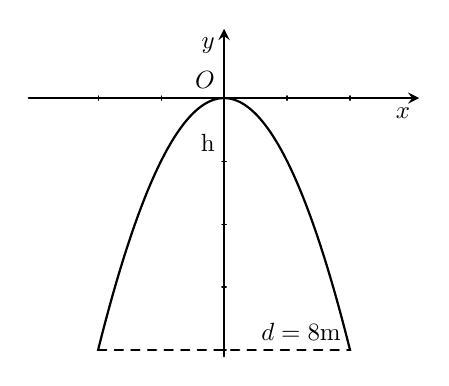
\begin{tikzpicture}[line join=round,line cap=round,>=stealth,thick,scale=0.8]
				\tikzset{every  node/.style={scale=0.9}}
				\draw[->]  (-3.1,0)--(3.1,0) node[below left] {$x$};
				\draw[->] (0,-4.1)--(0,1.1) node[below  left] {$y$};
				\draw[dashed] (-2,-4) --  (2,-4) node[above left] {$d=8$m};
				\draw (0,-1)  node[above left] {h};
				\draw (0,0)  node [above left] {$O$};
				\foreach  \x/\nx in {-2/-2,-1/-1,1/1,2/2}
				\draw[thin]  (\x,1pt)--(\x,-1pt);
				\foreach  \y/\ny in {-1/-1,-2/-2,-3/-3,-4/-4}
				\draw[thin] (1pt,\y)--(-1pt,\y); 
				\begin{scope}
					\clip (-3,-4) rectangle  (3,1);
					\draw[samples=200,domain=-3:3,smooth,variable=\x] plot  (\x,{-1*(\x)^2+0*(\x)+0});
				\end{scope}
			\end{tikzpicture}
		} 
	 \loigiai{
		Dựa vào hệ trục tọa độ hình minh họa $d=8$m suy ra đồ  thị hàm số đi qua điểm có tọa độ $(4; h)$ Suy ra $h=-4^2=-16$. Mà thực tế $h$ là chiều cao cổng nên $h=16$m.
	} 
\end{ex}

% nguồn: MaHoaNH_TracNghiem_Lop10
\begin{ex}%[0D3B2-6]%[ma:89f70466]
	Cho tập hợp $S=\left\{2;3;4;5;6;7;8\right\}$. Chọn ngẫu nhiên một số từ tập hợp $S$, tính xác suất để số  được chọn là số chẵn.
	 \choice
		 {$\dfrac{3}{8}$}
		 {\True $\dfrac{4}{7}$}
		 {$\dfrac{5}{7}$}
		{$\dfrac{3}{7}$} 
	\loigiai{Ta có $n\left(S  \right)=7$\\
		Gọi $A$ là biến cố  "số được chọn là số chẵn"\\
		Do  đó $n\left(A \right)=4 $\\
		Xác suất cần tìm là  $P\left(A \right)=\dfrac{n\left(A \right) }{n\left(S \right) }=\dfrac{4}{7} $
	 }
\end{ex}

% nguồn: MaHoaNH_TracNghiem_Lop10
\begin{ex}%[0D3B2-6]%[ma:ecd46391]
	Từ các chữ số $1$; $2$; $4$; $6$; $8$; $9$  lấy ngẫu nhiên một số. Xác suất để lấy được một số nguyên tố là
	\choice 
		{$\dfrac{1}{2}$} 
		{$\dfrac{1}{3}$} 
		{$\dfrac{1}{4}$} 
		 {\True $\dfrac{1}{6}$}
	 \loigiai{
		 Ta có $n(\Omega)=6$.\\
		Biến cố $A$ \lq\lq Lấy được một  số nguyên tố\rq\rq.\\
		 $A=\left\{2\right\}$, suy ra $n(A)=1$.\\
		Vậy xác suất biến cố $A$ là $\mathrm{P}(A)=\dfrac{n(A)}{n(\Omega)}=\dfrac{1}{6}$. 
	} 
\end{ex}

% nguồn: MaHoaNH_TracNghiem_Lop10
\begin{ex}%[0D3G2-6]%[ma:bf24bc7c]
	Gọi $S$ là tập hợp tất cả các số tự nhiên gồm $4$ chữ số khác nhau được chọn từ tập hợp  $A=\{1;2;3;4;5;6\}$. Chọn ngẫu nhiên một số từ tập hợp $S$. Tính xác suất để số được chọn có $2$ chữ số chẵn và $2$ chữ số lẻ.
	 \choice
		 {$\dfrac{2}{5}$}
		 {$\dfrac{1}{6}$}
		{\True  $\dfrac{3}{5}$}
		 {$\dfrac{1}{10}$}
	 \loigiai{
		Từ  tập $A=\{1;2;3;4;5;6\}$ ta lập được $\mathrm{A}_6^4=360$ số tự nhiên có $4$ chữ số khác nhau.\\
		Phép thử ``chọn một số trong $360$ số đó'' cho ta số phần tử không gian mẫu là $n(\Omega)=360$.\\ 
		Xét biến cố $X$: ``chọn được số có $2$ chữ số chẵn  và $2$ chữ số lẻ''.\\
		Số kết  quả thuận lợi cho $X$ là $n(X)=\mathrm{C}_3^2\cdot\mathrm{C}_3^2\cdot 4!=216$.\\
		 Vậy xác suất của $X$ là $\mathrm{P}(X)=\dfrac{216}{360}=\dfrac{3}{5}$.
	} 
\end{ex}

% nguồn: MaHoaNH_TracNghiem_Lop10
\begin{ex}%[0D3B2-6]%[ma:125bdab4]
	Cho tập hợp $A=\{0;1;2;3;4;5;6\}$ và $S$ là tập hợp các số tự nhiên có ba chữ số khác nhau được lập từ các chữ số của tập hợp $A$. Lấy ngẫu nhiên một số thuộc tập hợp $S$. Xác suất của biến cố: "Số được  chọn là một số chia hết cho $5$" là
	\choice 
		{$\dfrac{11}{35}$} 
		{$\dfrac{11}{42}$} 
		{\True $\dfrac{11}{36}$} 
		{$\dfrac{11}{24}$} 
	 \loigiai{
		Gọi số cần tìm trong tập $S$  có dạng $\overline{abc}$.\\
		 Ta có
		\begin{itemize}
			\item Chọn $a\in  A\setminus\{0\}$ có $6$ cách.
			\item Chọn $b\in A\setminus\{a\}$  có $6$ cách.
			\item Chọn  $c\in A\setminus\{a;b\}$ có $5$ cách.
		\end{itemize}
		Do đó tập $S$ có $6\cdot 6\cdot  5=180$ phần tử.\\
		Suy ra số phần tử của không gian mẫu là  $n(\Omega)=\mathrm{C}_{180}^1=180$.\\
		Gọi $X$ là biến cố \lq\lq Số được chọn là một số  chia hết cho $5$\rq\rq.\\
		Khi đó ta  có
		\begin{itemize}
			\item \textbf{TH1.} $c=0$.\\ 
			Số cách  chọn $\overline{ab}$ là $\mathrm{A}_{6}^2=30$ cách.\\
			Suy  ra trường hợp này có $30$ số chia hết cho $5$.
			\item  \textbf{TH2.} $c=5$.
			\begin{itemize}
				\item Chọn $a\in A\setminus\{0\}$ có $5$  cách.
				\item Chọn $b\in A\setminus\{a,  c\}$ có $5$ cách.
			\end{itemize}
			Suy ra trường hợp này có $5\cdot5=25$ số chia hết cho $5$. 
		\end{itemize}
		 Do đó số phần tử của biến cố $X$ là $n(X)=30+25=55$.\\
		Vậy xác suất cần  tính là $\mathrm{P}(X)=\dfrac{n(X)}{n(\Omega)}=\dfrac{55}{180}=\dfrac{11}{36}$.
	} 
\end{ex}


%%%%%%%%%%%%%%%% ĐÚNG/SAI %%%%%%%%%%%%%%%%

% nguồn: MaHoaNH_DungSai_Lop10
\begin{ex}%[0D3V2-6]%[ma:a007cb60]
	Một cửa hàng hoa quả bán dưa hấu với giá  $50\,000$ đồng một quả. Với mức giá này thì chủ cửa hàng nhận thấy họ chỉ bán được $40$ quả mỗi ngày. Cửa hàng nghiên cứu thị trường cho thấy, nếu giảm giá mỗi quả $1\,000$ đồng thì số dưa hấu bán mỗi ngày tăng thêm $2$ quả. Biết rằng giá nhập về của mỗi quả dưa là $20\,000$ đồng.
	\choiceTF 
		{\True Lợi nhuận  bán dưa mỗi ngày được biểu thị bằng tam thức $f(x)=-2x^{2}+20x+1\,200$}
		{Số lượng dưa bán ra khi giảm giá là $40$ trái} 
		{Lợi nhuận trên  mỗi trái dưa sau khi giảm giá $30\,000$ đồng}
		{\True Giá bán  mỗi quả dưa $45\,000$ đồng thì cửa hàng thu được lợi nhuận mỗi ngày cao nhất}
	 \loigiai{
		\begin{itemchoice}
			\itemch Gọi $x$  (nghìn đồng, $0<x<30$) là số tiền giảm giá.\\
			Số lượng dưa  bán ra khi giảm giá là $40+2x$ (trái).\\
			 Lợi nhuận trên mỗi trái dưa sau khi giảm giá là $30-x$ (nghìn đồng).\\
			Lợi nhuận bán dưa mỗi ngày là $(40+2x)(30-x)=-2x^{2}+20x+1\,200$ (nghìn đồng). 
			\itemch Xét hàm số  $f(x)=-2x^{2}+20x+1\,200$ trên khoảng $(0;30)$.\\
			Do hàm số có hệ số $a=-2<0$ nên hàm số  đạt giá trị lớn nhất tại $x=-\dfrac{b}{2a}=5$.\\
			Số lượng dưa bán ra  khi giảm giá là $40+2\cdot5=50$ (trái).
			\itemch Lợi nhuận trên  mỗi trái dưa sau khi giảm giá là $30-5=25$ (nghìn đồng).
			 \itemch Vậy cửa hàng cần giảm giá $5\,000$ đồng cho mỗi quả để đạt được lợi nhuận cao nhất.\\
			Vậy giá bán mỗi quả dưa cần tìm  là $45\,000$ đồng.
		\end{itemchoice}
	} 
\end{ex}

% nguồn: MaHoaNH_DungSai_Lop10
\begin{ex}%[0D3V2-6]%[ma:f132b837]
	Một cửa hàng hoa quả bán dưa hấu với giá $50\,000$ đồng một quả. Với mức giá này thì chủ cửa hàng nhận thấy họ chỉ bán được $40$ quả mỗi ngày. Cửa hàng nghiên cứu thị trường cho thấy, nếu giảm giá mỗi quả $1\,000$ đồng thì số dưa hấu bán mỗi ngày tăng thêm $2$ quả. Biết rằng giá nhập về của mỗi quả dưa là $20\,000$ đồng. Cho  biết tính đúng sai của các khẳng định dưới đây.
	 \choiceTF
		{Số lượng dưa bán ra khi giảm giá  là $40$ trái}
		{Lợi nhuận trên mỗi trái dưa sau khi  giảm giá $30\,000$ đồng}
		{\True Lợi nhuận bán dưa  mỗi ngày được biểu thị bằng tam thức $f(x)=-2 x^2+20 x+1\,200$}
		 {\True Giá bán mỗi quả dưa $45\,000$ đồng thì cửa hàng thu được lợi nhuận mỗi ngày cao nhất}
	\loigiai{ 
		Gọi $x$ (nghìn đồng) là số tiền giảm  giá (điều kiện $0<x<30$).\\
		 Số lượng dưa bán ra khi giảm giá $40+2 x$ (trái).\\
		Lợi nhuận trên mỗi  trái dưa sau khi giảm giá $30-x$ (nghìn đồng).\\
		Lợi  nhuận bán dưa mỗi ngày là $(40+2 x)(30-x)=-2 x^2+20 x+1\,200$ (nghìn đồng).\\
		Xét hàm số  $f(x)=-2 x^2+20 x+1\, 200$ trên khoảng $(0; 30)$.\\
		Do hàm số có hệ  số $a=-2<0$ nên hàm số đạt giá trị lớn nhất tại $x=-\dfrac{b}{2 a}=5$.\\
		Vậy cửa hàng cần giảm giá $5\,000$ đồng cho mỗi quả để đạt được lợi nhuận cao  nhất.\\
		 Vậy giá bán mỗi quả dưa cần tìm là $45\,000$ đồng.
		\begin{itemchoice}
			\itemch \textbf{ Sai}. Vì  số lượng dưa bán ra khi giảm giá là $50$ trái.
			\itemch \textbf{ Sai}. Vì lợi nhuận  trên mỗi trái dưa sau khi giảm giá là $25\,000$ đồng.
			\itemch \textbf{ Đúng}. Vì lợi nhuận bán dưa mỗi ngày  được biểu thị bằng tam thức $f(x)=-2 x^2+20 x+1\,200$.
			\itemch \textbf{ Đúng}. Vì giá bán mỗi quả  dưa $45\,000$ đồng thì cửa hàng thu được lợi nhuận mỗi ngày cao nhất.
		\end{itemchoice}
	} 
\end{ex}


%%%%%%%%%%%%%%%% TRẢ LỜI NGẮN %%%%%%%%%%%%%%%%

% nguồn: MaHoaNH_TraLoiNgan_Lop10
\begin{bt}%[0D3H2-6]%[ma:cd8da407]
	 Một cửa hàng kinh doanh giày và giá để nhập một đôi giày là $40$ đô la. Theo nghiên cứu của bộ phận kinh doanh thì nếu cửa hàng bán mỗi đôi giày với giá $x$ đô la thì mỗi tháng sẽ bán được $120-x$ đôi giày. Hỏi cửa hàng bán giá bao nhiêu cho một đôi giày để có thể thu lãi cao nhất trong tháng.
	 \shortans{1600}
	 \loigiai{
		Gọi $x$ (đô la) là giá mỗi đôi giày bán  ra thì số tiền lãi tương ứng là $x-40$ (đô la) Số tiền lãi thu được mỗi tháng là $f(x)=(x-40)(120-x)=-x^2+160 x-4800$.\\
		Đây là hàm số bậc hai với $a=-1$, $b=160$, $c=-4800 \Rightarrow-\dfrac{b}{2 a}=80$.\\ 
		Vì $a=-1<0$ nên hàm số đạt giá  trị lớn nhất bằng $f(80)=-80^2+160\cdot80-4800=1600$, ứng với $x=80$.\\
		Vậy, để tối ưu hóa lợi nhuận, cửa hàng cần đưa ra giá bán  80 đô la mỗi đôi giày, khi đó lợi nhuận tối đa trong tháng là 1600 đô la.
	 }
\end{bt}

% nguồn: MaHoaNH_TraLoiNgan_Lop10
\begin{bt}%[0D3H2-6]%[ma:3b5b90f7]
	Một quả bóng được đá lên từ độ cao $1{,}5$ mét so với mặt đất. Biết quỹ đạo  của quả bóng là một đường parabol trong mặt phẳng tọa độ $Oxy$ có phương trình $h=at^2+bt+c$ ($a<0$) trong đó $t$ là thời gian (tính bằng giây) kể từ khi quả bóng được đá lên và $h$ là độ cao (tính bằng mét) của quả bóng. Biết rằng sau $2$ giây thì nó đạt độ cao $5$ m; sau $4$ giây thì nó đạt độ cao $4{,}5$ m. Hỏi sau $5{,}5$ giây quả bóng đạt độ cao bao nhiêu mét so với mặt đất? Viết kết quả dưới dạng số thập phân.
	 \shortans{1,5}
	\loigiai{ 
		 Theo giả thiết, ta có hệ phương trình sau
		$$\heva{&h(0)=\dfrac{3}{2}\\&h(2)=5\\&h(4)=\dfrac{9}{2}}\Leftrightarrow \heva{&a\cdot 0^2+b\cdot 0+c=\dfrac{3}{2}\\&a\cdot  2^2+b\cdot 2+c=5\\&a\cdot 4^2+b\cdot 4+c=\dfrac{9}{2}}\Leftrightarrow \heva{&c=\dfrac{3}{2}\\&4a+2b+c=5\\&16a+4b+c=\dfrac{9}{2}}\Leftrightarrow \heva{&a=-\dfrac{1}{2}\\&b=\dfrac{11}{4}\\&c=\dfrac{3}{2}.}$$
		Suy ra $h=-\dfrac{1}{2}t^2+\dfrac{11}{4}t+\dfrac{3}{2}$.  \\
		Khi $t=5{,}5$ suy ra  $h=1{,}5$.\\
		Vậy sau $5{,}5$ giây thì quả bóng đạt độ cao $1{,}5$ mét so  với mặt đất.
	} 
\end{bt}

% nguồn: MaHoaNH_TraLoiNgan_Lop10
\begin{bt}%[0D3H2-6]%[ma:8247738b]
	\immini  {
	Có một chiếc cổng hình Parabol. Người ta đo khoảng cách giữa hai chân cổng $BC$ là $8$ m.  Từ một điểm $M$ trên thân cổng người ta đo được khoảng cách tới mặt đất là $MK=21$ m và khoảng cách tới chân cổng gần nhất là $BK=1$ m. Khi đó chiều cao của cổng bằng bao nhiêu mét?
	\shortans {48} 
	}{ 
	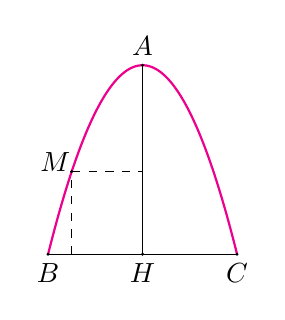
\begin{tikzpicture}[smooth,samples=300,scale=0.6,>=stealth]
			\draw[]  (-2,0)--(2,0);
			\draw[]  (0,0)--(0,4);
			\draw[thick,magenta,domain=-2:2] plot  (\x,{-1*(\x)^2+4});
			\draw[dashed]  (-1.5,0)|-(0,1.75);
			 \foreach \x/\y/\t/\g in {0/4/A/90,-2/0/B/-90,2/0/C/-90,-1.5/1.75/M/150,0/0/H/-90}
			\fill[black] (\x,\y) circle (1pt)+(\g:4mm)  node[scale=1]{$\t$};
		\end{tikzpicture}
	} 
	 \loigiai{
		Chọn hệ trục tọa độ sao cho trục tung đi qua $AH$, trục hoành đi qua  $BH$ như hình vẽ.
		\begin{center}
			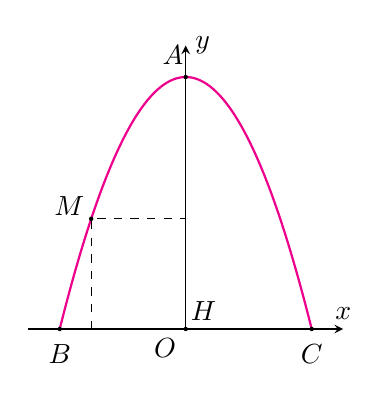
\begin{tikzpicture}[smooth,samples=300,scale=0.8,>=stealth]
					\draw[->]  (-2.5,0)--(2.5,0) node[above]{$x$};
					\draw[->] (0,0)--(0,4.5) node[right]{$y$}; 
					\draw (0,0) node[below  left]{$O$};
					\draw[thick,magenta,domain=-2:2] plot (\x,{-1*(\x)^2+4}); 
					\draw[dashed] (-1.5,0)|-(0,1.75); 
					\foreach \x/\y/\t/\g  in {0/4/A/120,-2/0/B/-90,2/0/C/-90,-1.5/1.75/M/150,0/0/H/45}
					\fill[black] (\x,\y)  circle (1pt)+(\g:4mm) node[scale=1]{$\t$};
				\end{tikzpicture}
		\end{center}
		Hình  dạng cái cổng là một Parabol đi qua các điểm như hình vẽ.\\
		 Khi đó theo giả thiết các điểm $B(-4;0)$, $C(4;0)$, $H(0;0)$ và $M(-3;21)$.\\
		Do Parabol nhận trục tung làm trục đối xứng nên phương trình có dạng  $y=ax^2+c$ ($a \ne 0$).\\
		Parabol đi qua $B(-4;0)$,  $C(4;0)$ và $M(-3;21)$ nên ta có hệ
		$$\heva{&16a+c=0 \\ &9a+c=21} \Leftrightarrow \heva{&a=-3 \\&c=48.}$$ 
		 Vậy phương trình Parabol là $y=-3x^2+48$.\\
		Khi đó  $A(0;48)$ là đỉnh của Parabol.\\
		Suy  ra chiều cao cái cổng là $AH=48$ (m).
	} 
\end{bt}

% nguồn: MaHoaNH_TraLoiNgan_Lop10
\begin{bt}%[0D3V2-6]%[ma:5dacdd9b]
	Một quả bóng được đá lên từ độ cao $1{,}5$ mét so với mặt đất. Biết quỹ đạo của quả bóng là một đường parabol trong mặt phẳng tọa độ $Oxy$ có phương trình là $h=a t^2+b t+c~(a < 0)$ trong đó $t$ là thời gian (tính bằng giây) kể từ khi quả bóng được đá lên và $h$ là độ cao (tính bằng  mét) của quả bóng. Biết rằng sau 2 giây thì nó đạt độ cao $5 \mathrm{~m}$; sau 4 giây nó đạt độ cao $4{,}5$ m. Hỏi sau $5{,}5$ giây quả bóng đạt độ cao bao nhiêu mét so với mặt đất?
	 \shortans{1,5}
	 \loigiai{
		 Chọn hệ trục tọa độ $Oxy$ với trục $Ox$ là trục thời gian.\\
		Theo đề bài ta có hệ phương trình  sau $\heva{&c=1{,}5\\&4a+2b+c=5\\&16a+4b+c=4{,5}}\Leftrightarrow \heva{&a=-\dfrac{1}{2}\\&b=\dfrac{11}{4}\\&c=\dfrac{3}{2}.}$\\
		Do đó phương  trình quỹ đạo của quả bóng là $y=-\dfrac{1}{2}t^2+\dfrac{11}{4}t+\dfrac{3}{2}$.\\
		Vậy sau $5{,}5$ giây quả bóng đạt độ  cao $h=y(5{,}5)=1{,}5$ m.
	 }
\end{bt}

% nguồn: MaHoaNH_TraLoiNgan_Lop10
\begin{bt}%[0D3V2-6]%[ma:d922b30d]
	Một trận bóng đá được tổ chức ở một sân vận động có sức chứa $15\,000$ người. Với giá vé $14$ \$ thì trung bình các trận đấu gần đây có $9\,500$ khán giả. Theo một khảo sát thị trường đã chỉ ra rằng cứ giả $1$ \$ mỗi vé thì trung bình số khán giả tăng lên $1\,000$ người. Giá  vé bằng bao nhiêu thì thu được nhiều lợi nhuận nhất (đơn vị: \$)? Kết quả làm tròn đến hàng phần mười.
	 \shortans{11,8}
	 \loigiai{
		Ta thấy có hai  đại lượng thay đổi là giá vé và số lượng khán giả.\\
		Gọi $x$ \$ là giá  vé $(x>0)$.\\
		Số tiền  giá vé được giảm xuống là $14-x$.\\
		Số khán  giả tăng lên là $1000(14-x)$.\\
		Số  khán giả là $9\,500+1\,000(14-x)$.\\
		Do lợi nhuận bằng giá vé nhân với số khán giả nên nếu gọi lợi nhuận  thu được là $y$ thì
		 $$
		y=x(9\,500+1\,000(14-x))=-1\,000 x^2+23\,500  x.
		$$ 
		Do $y$ là  tam thức bậc hai nên nhận giá trị cực đại khi $x=\dfrac{-b}{2 a}=\dfrac{-23\,500}{-2\,000}=11{,}75$.\\
	Vậy giá vé bằng $11{,}8$ \$ thì thu được  nhiều lợi nhuận nhất.}
\end{bt}

% nguồn: MaHoaNH_TraLoiNgan_Lop10
\begin{bt}%[0D3V2-6]%[ma:d7cf2702]
	Trong một đám cháy rừng, các máy bay trực thăng cứu hộ được điều động để phun nước dập tắt các đám cháy. Một chiếc trực thăng  mang số hiệu CH01 đang bay ở độ cao $500$ m so với mặt đất, chuẩn bị phun nước vào một đám cháy rừng từ trên cao. Độ cao $h$ (m) của vòi phun so với mặt đất tính theo thời gian $t$ (s) kể từ lúc máy bay phun ra nước để dập lửa là một hàm số bậc hai. Tại thời điểm $5$ s sau khi nước phun thì nước tới được phía trên đám cháy đang bốc lửa cao $90$ m. Khoảng thời gian để nước đi từ vòi phun đến đám cháy trên mặt đất đạt bao nhiêu giây? Kết quả làm tròn đến hàng phần mười.
	 \shortans{5,5}
	\loigiai{ 
	\immini{Chọn hệ trục $Oth$ như hình vẽ với gốc tọa độ $O$ là vị trí trên mặt đất thẳng đứng  với trực thăng.\\
		 Xét phương trình parabol $(P)\colon h(t)=a t^2+b t+c$, $a \neq 0$ mô tả độ cao của vòi phun so với mặt đất.\\
		Theo giả thiết, ta có tọa độ của trực thăng là $S(0; 500)$ và $(P)$ đi qua điểm $A(5; 90)$. Đỉnh $S(0; 500)$ của $(P)$ nằm trên trục tung nên $(P)\colon  h(t)=a t^2+500$.\\
		Mặt khác, $A(5; 90)  \in(P)$ nên $a=-16{,}4$. Từ đây ta được phương trình $(P)\colon h(t)=-16{,}4t^2+500$.\\
		Khi nước chạm  đất ta được $\heva{&t > 0\\&h(t)=0} \Leftrightarrow\heva{&t > 0\\&-16{,}4t^2+500=0} \Leftrightarrow t \approx 5{,}5$ s.\\
		Vậy thời gian để  nước đi từ vòi phun đến đám cháy trên mặt đất xấp xỉ $5{,}5$ s.}{
		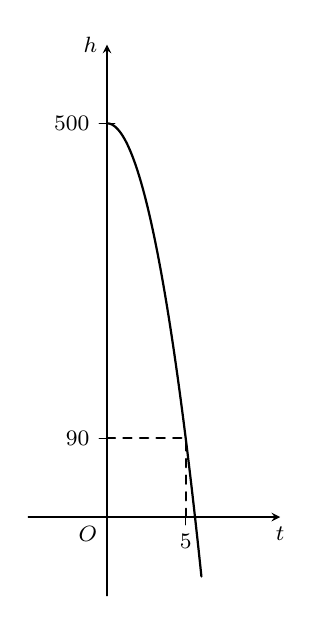
\begin{tikzpicture}[line join = round,line cap = round,>=stealth,font=\footnotesize,scale=1]
				 \def\a{-4}
				 \def\b{0}
				\def\c{5} 
				 \def\f (#1){\a*((#1)^2)+\b*(#1)+\c}
				\def\xmin{0} 
				\def\xmax{1.2} 
				\def\ymin{0} 
				 \def\ymax{5}
				\draw[->] (\xmin-1,0)--(\xmax+1,0)  node[below] {$t$};
				 \draw[->] (0,\ymin-1)--(0,\ymax+1) node[left] {$h$};
				\draw (0,0) node [below left] {$O$}; 
				\draw (1,0.1)--(1,-0.1) node [below] {$5$}; 
				\draw (0.1,1)--(-0.1,1) node  [left] {$90$};
				\draw (0.1,5)--(-0.1,5) node  [left] {$500$};
				\draw[thick,smooth,samples=200] plot[domain=\xmin:\xmax] (\x,{\f (\x)}); 
				\draw[dashed,thick]  (1,0)--(1,1)--(0,1);
			\end{tikzpicture}
		} 
	 }
\end{bt}

% nguồn: MaHoaNH_TraLoiNgan_Lop10
\begin{bt}%[0D3V2-6]%[ma:230636cd]
	\immini[thm]{Một viên bi được ném xiên từ vị trí $A$ cách mặt đất $2\mathrm{\,m}$ theo quỹ đạo dạng parabol như hình vẽ bên. Tìm khoảng cách từ vị trí $E$ đến vị trí $F$,  biết vị trí $E$ là nơi viên bi rơi xuống chạm mặt đất (kết quả làm tròn đến số thập phân thứ hai).}
	{ 
	\begin{tikzpicture}[scale=1,line join=round,font=\footnotesize,line cap=round,>=stealth,yscale=0.7]
			\draw[->] (0,0)--(3,0)  node[below] {$x$};
			\draw[->]  (0,0)--(0,8) node[left] {$y$};
			\draw (0,0) node  [below left] {$O$};
			\foreach \x/\nx in {1/1} 
			\draw[thin] (\x,1pt)--(\x,-1pt) node  [below] {$\nx$};
			 \foreach \y/\ny in {2/2,3/3,4/4,5/5,6/6,7/7}
			\draw[thin] (1pt,\y)--(-1pt,\y) node  [left] {$\ny$};
			 \draw[dashed,thin](1,0)--(1,7)--(0,7);
			\begin{scope}
				\clip  (-1,-1) rectangle (3,8);
				\draw[samples=200,domain=0:2.183,smooth,variable=\x] plot (\x,{-5*(\x)^2+10*(\x)+2}); 
				\path (0,2) node[right]{$A$}; 
				\path  (1,7) node[above]{$C$};
				 \path (2.183,0) node[below]{$E$};
				\path  (0,0) node[above right]{$F$};
				 \fill (0,0) circle (1pt)
					(1,7) circle  (1pt)
					 (0,2) circle (1pt)
					(2.183,0) circle  (1pt);
			\end{scope}
		\end{tikzpicture}
	 }
	 \shortans{2,18}
	\loigiai{ 
		Đặt hệ trục tọa độ $Oxy$ sao cho điểm $F$ trùng với gốc tọa độ $O$ và điểm $A$  thuộc tia $Oy$, điểm $E$ thuộc tia $Ox$.\\
		Gọi parabol  có dạng $(P)\colon y=ax^2+bx+c\,(a\ne 0)$.\\
		Ta có  $A(0;2)\in (P)\Rightarrow c=2$.\\
		Hoành độ đỉnh  $x=-\dfrac{b}{2a}=1\Rightarrow 2a+b=0.\,(1)$\\
		$C(1,7)\in (P)\Rightarrow a+b+c=7\Rightarrow a+b=5.\,(2)$\\ 
		 Từ $(1)$ và $(2)\Rightarrow a=-5, b=10$.\\
		Vậy $(P)\colon  y=-5x^2+10x+2$.\\
		Ta có $E(x,0)\in (P)\Rightarrow -5x^2+10x+2=0\Rightarrow \hoac{&x=\dfrac{5+\sqrt{35}}{5}\\&x=\dfrac{5-\sqrt{35}}{5}.}$\\ 
		Do $E$ thuộc tia $Ox$ nên $x>0\Rightarrow  x=\dfrac{5+\sqrt{35}}{5}\approx 2{,}18$.\\
		 Vậy $EF\approx 2{,}18$.
	 }
\end{bt}
